\documentclass[14pt, a4paper]{extreport}

\usepackage{susu}

% ====================================================================================================
\begin{document}

\author{Исрафилова~Д.В.}
\group{213}
\task{5}
\maketitle

% ====================================================================================================
\chapter{Задание}

    \par
    Написать программу для построения гладкой кривой по четырем опорным точкам. При выборе опорных точек текущие координаты указателя мыши должны отображаться в графическом окне. Интерфейс программы должен содержать следующие элементы управления:
    \begin{itemize}
		\item выбор опорных точек;
		\item построение кубической кривой Безье;
		\item построение кривой по алгоритму Чайкина;
        \item сохранение результата в файл;
        \item выход из программы.
	\end{itemize}
	



% ====================================================================================================
\chapter{Математическая модель}
\begin{enumerate}
    \item Математическая модель алгоритма для построения Кривой Безье.
Пусть $P_0(x_0,y_0), P_1(x_1,y_1), P_2(x_2,y_2), P_3(x_3,y_3)$ - точки, которые определяют кривую Безье. 
Последующие координаты $x,y$ находятся по формулам:
$$P = (1 - z)^3x_0 + 3(1 - z)^2zx_1 + 3(1 - z)z^2x_2 + z^3x_3,$$
$$P = (1 - z)^3y_0 + 3(1 - z)^2zy_1 + 3(1 - z)z^2y_2 + z^3y_3.$$
    \item Математическая модель алгоритма для построения кривой по алгоритму Чайкина.
Пусть $P_0(x_0,y_0), P_1(x_1,y_1), P_2(x_2,y_2), P_3(x_3,y_3)$ - точки, выбранные для 
построения кривой Чайкина.
На каждой итерации на отрезке ломанной между точками $P_i$ и $P_{i+1}$ выбираютя две новые точки $Q_i$ $R_i$, которые вычисляются по формулам:
$$Q_i = 0,75P_i + 0.25P_{i+1},$$
$$R_i = 0,75P_i + 0.25P_{i+1}.$$
Точки $P_i$ и $P_{i+1}$ удаляются.
\end{enumerate}
% ====================================================================================================
\chapter{Текст программы}

\noindent Файл main.cpp
\lstinputlisting{source/main.cpp}
\pagebreak
\hrulefill

\noindent Файл task.h
\lstinputlisting{source/task.h}
\hrulefill

\noindent Файл task.cpp
\lstinputlisting{source/task.cpp}
\hrulefill

\noindent Файл control.h
\lstinputlisting{source/control.h}
\hrulefill

\noindent Файл control.cpp
\lstinputlisting{source/control.cpp}

% ====================================================================================================
\chapter{Результат работы}

\begin{figure}[h!]
	\centering
	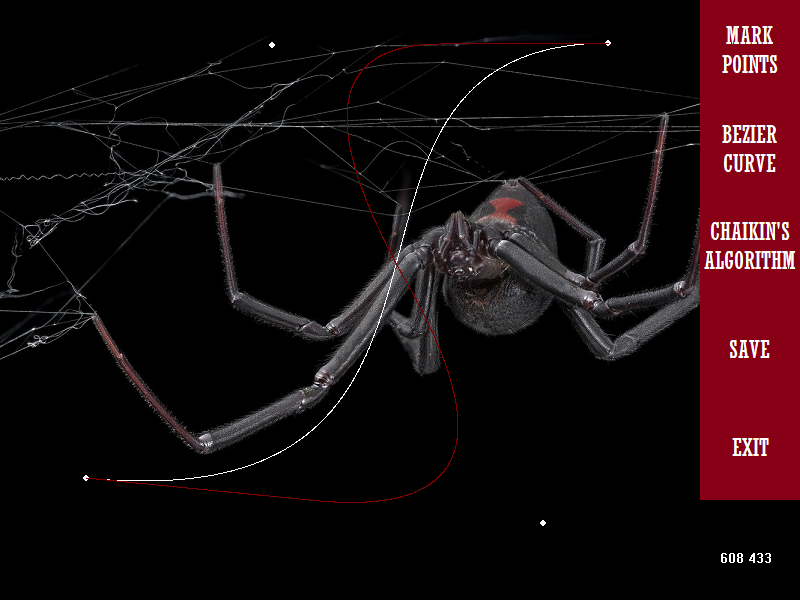
\includegraphics[width = 13cm]{image/image_1}
  \caption{Результат выполнения программы}
\end{figure}
\begin{figure}[h!]
	\centering
	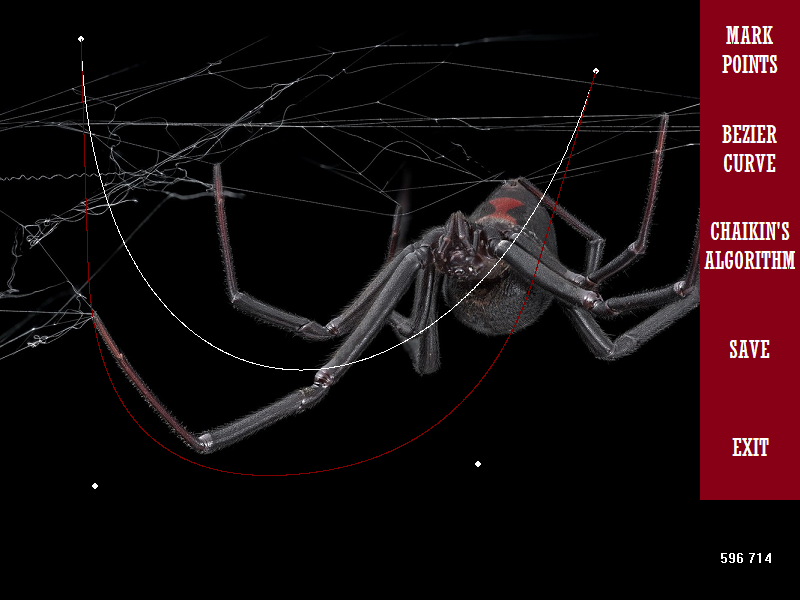
\includegraphics[width = 13cm]{image/image_2}
  \caption{Результат выполнения программы}
\end{figure}
\begin{figure}[h!]
	\centering
	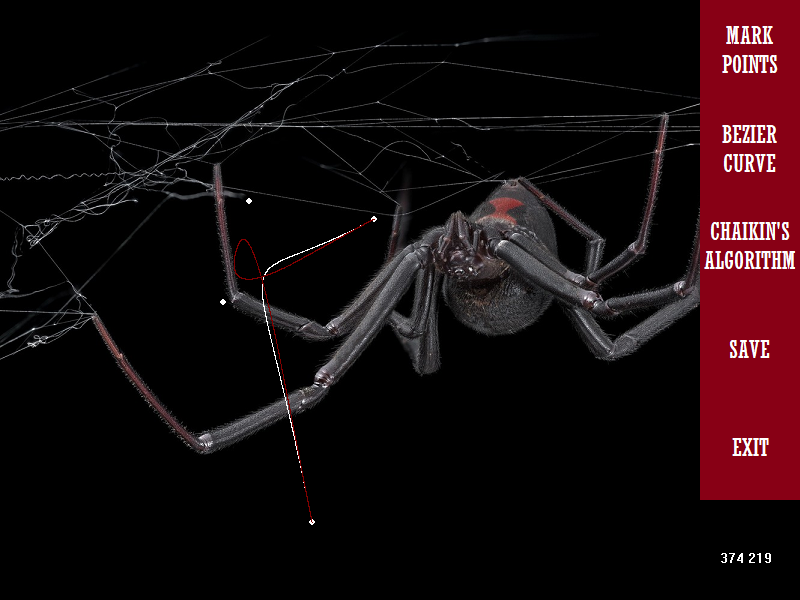
\includegraphics[width = 13cm]{image/image_3}
  \caption{Результат выполнения программы}
\end{figure}
\begin{figure}[h!]
	\centering
	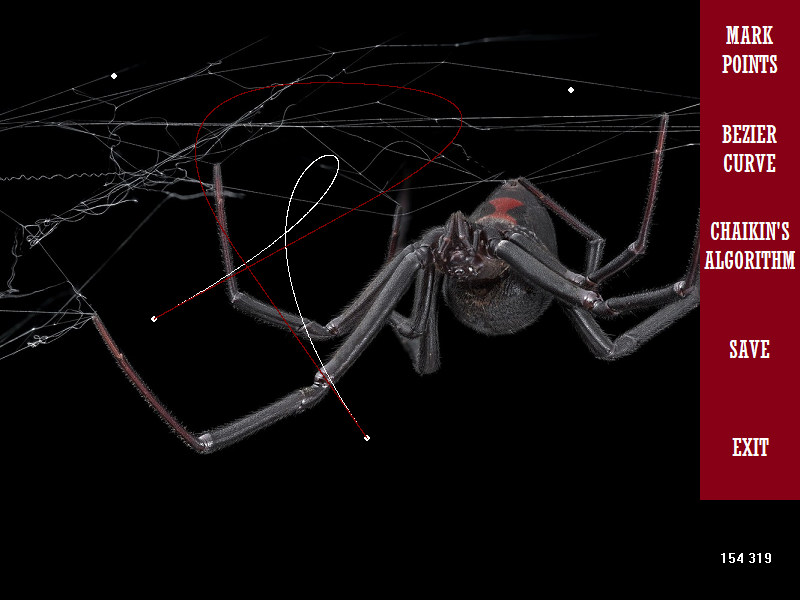
\includegraphics[width = 13cm]{image/image_4}
  \caption{Результат выполнения программы}
\end{figure}
% ====================================================================================================
\end{document}